
\documentclass{beamer}

\usepackage[utf8]{inputenc}
\usepackage[slovak]{babel}
\usepackage{beamerthemeshadow}
\usetheme{Warsaw}
\usecolortheme{default}
\usefonttheme{professionalfonts}
\useinnertheme{rectangles}
\begin{document}

\title{Besselove funkcie}  
\author{Peter Haspra, Ivan Turiak, Peter Žuffa}
\date{\today} 

\begin{frame}
\titlepage
\end{frame}

\begin{frame}\frametitle{Obsah}\tableofcontents
\end{frame} 

\section{Besselove funkcie} 

\begin{frame}\frametitle{Úvod}

\begin{itemize}
\item Daniel Bernoulli, Friedrich Bessel
\item kanonické riešenie y(x) diferenciálnej rovnice
\end{itemize}
\begin{center}
$x^2\dfrac{d^2y}{dx^2}+x\dfrac{dy}{dx}+(x^2-\alpha^2)y=0$
\end{center}

\begin{itemize}
\item komplexne združené korene
\end{itemize}
\end{frame} 

\begin{frame}
\frametitle{Použitie Besselovej funkcie}
\begin{itemize}
\item vznikla pri hľadaní riešení Laplaceovej rovnice vo valcových alebo sférických súradniciach
\item šírenie elektromagnetických vĺn vo valcovom priestore
\item vedenie tepla vo valcových objektoch
\item spôsoby chvenia okrúhlych alebo oválnych membrán
\item riešenie vzorov akustického žiarenia
\item užitočné vlastnosti pre spracovanie signálov
\end{itemize}
\end{frame}

\begin{frame}
\frametitle{Definícia}
\begin{itemize}
\item diferenciálna rovnica druhého rádu
\item dve lineárne nezávislé riešienia
\item rôzne riešenia v závislosti od rôznych okolností
\end{itemize}

\end{frame}
\section{Besselova funkcia prvého druhu: $J_{\alpha}$}
\begin{frame}
\frametitle{Besselova funkcia prvého druhu: $J_{\alpha}$}
\begin{itemize} 
\item Riešenie Besselovej diferenciálnej rovnice definované Maclaurinovym radom
\end{itemize}
\begin{center}
$J_{\alpha}(x) = \displaystyle\sum\limits_{m=0}^{\infty}\dfrac{(-1)^m}{m!\Gamma(m+\alpha+1)}(\dfrac{1}{2}x)^{2m+\alpha} $

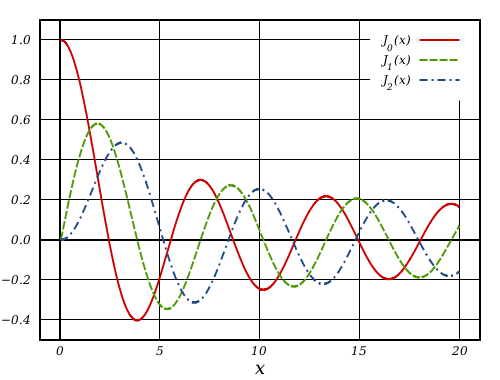
\includegraphics[height=120px]{bessel1.png} 
\end{center}
\end{frame}

\begin{frame}
\frametitle{Gama funkcia}

\begin{itemize}
\item Faktoriál pre všetky neceločíselné hodnoty
\item $\Gamma(z+1)=z!$
\item definícia:
\end{itemize}
\begin{center}
$ \Gamma(z) = \displaystyle\int\limits_{0}^{\infty}t^{z-1}e^{-t} dt$
\end{center}
\end{frame}

\begin{frame}
\frametitle{Besselova funkcia prvého druhu: $J_{\alpha}$}
\begin{itemize}
\item Oscilujúca funkcia
\item $J_{\alpha}(x)$ $J_{-\alpha}(x)$ Lineárne nezávislé pre neceločíselné hodnoty $\alpha$
\item  pre celočíselné $\alpha$ - Lineárne závislé (druhá Besselova funkcia)
\end{itemize}

\end{frame}

\begin{frame}
\frametitle{Besselove integrály}

Pre celočíselné $n$ je možné použiť integrál:

\begin{center}
$J_{n}(x) =  \dfrac{1}{\pi}\displaystyle\int\limits_{0}^{\pi} cos(n\tau - x sin \tau) d\tau$
\end{center} alebo
\begin{center}
$J_{n}(x) =  \dfrac{1}{2\pi}\displaystyle\int\limits_{-\pi}^{\pi} e^{-i(n\tau - x sin \tau)}d\tau$
\end{center}
\end{frame}
\section{Besselova funkcia druhého druhu: $Y_{\alpha}$}
\begin{frame}
\frametitle{Besselova funkcia druhého druhu: $Y_{\alpha}$}
\begin{center}
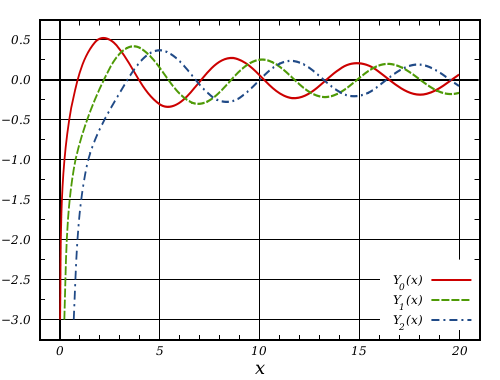
\includegraphics[scale=0.4]{bessel2.png} 
\end{center}
\end{frame}

\begin{frame}
\frametitle{Besselova funkcia druhého druhu: $Y_{\alpha}$}
\begin{itemize}
\item Nazývaná aj Neumannova funkcia
\item Vo vzťahu k $J_{\alpha}(x)$ 
\end{itemize}
\begin{center}
$Y_{\alpha}(x) = \dfrac{J_{\alpha}(x)cos(\alpha\pi)-J_{-a}(x)}{sin(\alpha\pi)} $
\end{center}
\begin{itemize}
\item limita, neceločíselné $\alpha$ sa blíži k celočíselnému $n$
\end{itemize}

\begin{center}
$Y_{n}(x) = \displaystyle\lim_{a\rightarrow n} Y_{\alpha}(x)$
\end{center}
$Y_{\alpha}(x) $ je potrebná ako druhé lineárne nezávislé riešenie $J_{\alpha}(x)$ v prípade, že $\alpha$ je celé číslo.
\end{frame}
\begin{frame}
\frametitle{Besselova funkcia druhého druhu: $Y_{\alpha}$}
\begin{itemize}
\item $J_{\alpha}(x)$ a $Y_{\alpha}(x)$ sú holomorfné funkcie

\item V prípade, že $\alpha$ je celé číslo, $J_{\alpha}$ je celá funkcia $(x)$.
Ak $x$ je konštantné, $J_{\alpha}$ a $Y_{\alpha}$ je celá funkcia $(\alpha)$.
\end{itemize}

\end{frame}

\section{Hankelove funkcie}
\begin{frame}
\frametitle{Hankelove funkcie}
\begin{itemize}
\item podľa Hermanna Hankela
\end{itemize}
\begin{center}
$H_{\alpha}^{(1)}(x) = J_{\alpha}(x) + iY_{\alpha}(x)$\\
$H_{\alpha}^{(2)}(x) = J_{\alpha}(x) - iY_{\alpha}(x)$
\begin{itemize}
\item tzv. Besselova funkcia tretieho druhu
\item skôr teoretický význam

\end{itemize}
\end{center}

\end{frame}

\section{Modifikované Besselove funkcie}
\begin{frame}
\frametitle{Modifikované Besselove funkcie}
\begin{itemize}
\item špeciálny prípad
\item čisto imaginárny argument
\item dve alternatívy
\end{itemize}
\begin{center}
$I_{\alpha}(x) =i^{-\alpha}J_{\alpha}(ix) = \displaystyle\sum\limits_{m=0}^{\infty}\dfrac{1}{m!\Gamma(m+\alpha+1)}(\dfrac{1}{2}x)^{2m+\alpha} $\\
\mbox{
$K_{\alpha}(x) = \dfrac{\pi}{2}\dfrac{I_{-\alpha}(x)-I_{\alpha}(x)}{sin(\alpha\pi)} = \dfrac{\pi}{2} i^{\alpha+1}H_{\alpha}^{(1)}(ix)=\dfrac{\pi}{2} (-i)^{\alpha+1}H_{\alpha}^{(2)}(-ix)$},

\end{center}
 kde $x\in R, x>0$
 \end{frame}
 \begin{frame}
$I_{\alpha}(x)$ a $K_{\alpha)}(x)$ sú dve lineárne nezávislé riešenia Besselovej rovnice.
\begin{itemize}
\item exponenciálne rastúce, resp. klesajúce funkcie
\item rozdiel medzi klasickou a modifikovanou besselovou funkciou
\end{itemize}
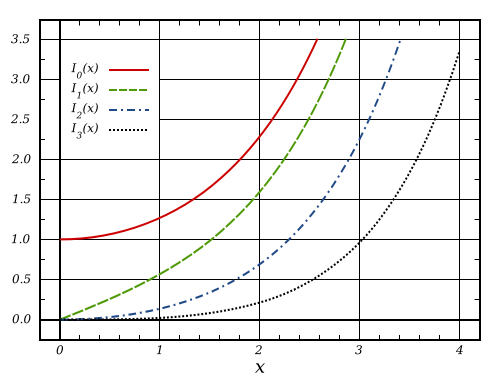
\includegraphics[scale=0.3]{bessel3.png} 
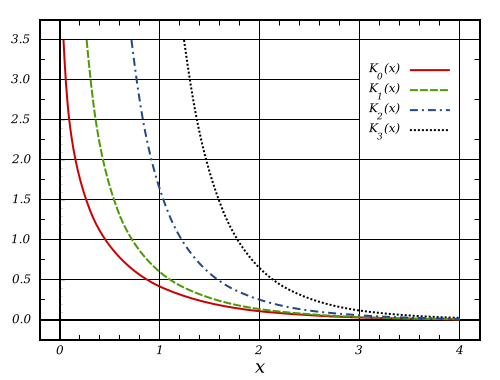
\includegraphics[scale=0.3]{bessel4.png} 
\end{frame}

\end{document}